\documentclass{beamer}

\usecolortheme[light]{solarized}

\beamertemplatenavigationsymbolsempty


\usepackage{booktabs}
\usepackage{graphicx}
\usepackage{hyperref}
\usepackage{minted}
\usepackage{moresize}
\usepackage{centernot}
\usepackage{standalone}
\usepackage{tcolorbox}
\usepackage{tikz}
\usepackage[normalem]{ulem}
\usepackage{xpatch}
\usepackage{fix-cm}

\xpatchcmd{\sout}
  {\bgroup}
    {\bgroup\def\ULthickness{2pt}}
      {}{}

\usetikzlibrary{calc, patterns}
\usetikzlibrary{arrows}
\usetikzlibrary{decorations.markings}
\usetikzlibrary{decorations.text}

\definecolor{twitter}{RGB}{64, 153, 255}
\definecolor{github}{RGB}{211, 211, 211}

\begin{document}

    \begin{frame}
        \begin{center}
            \Huge
                Ertai

               \vfill

            \Large
               Vince: \href{https://twitter.com/drvinceknight}{@drvinceknight}\\
        \end{center}

        % Hello, this will be a talk about a small python library called
        % "Ertai".
    \end{frame}

    \begin{frame}
        \begin{center}
            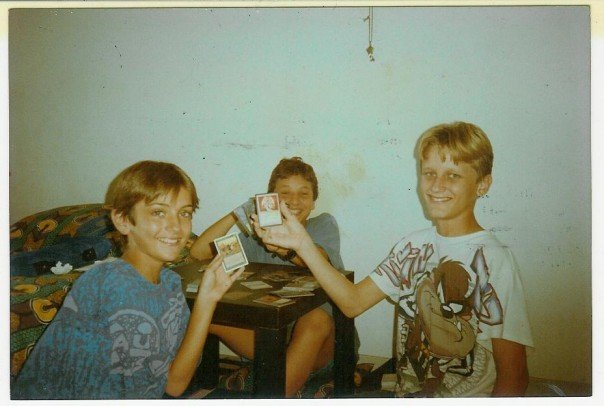
\includegraphics[width=.8\textwidth]{./img/young_me_playing_magic/main.jpg}
        \end{center}

        % My name is Vince, I'm the one on the right in the photo...
    \end{frame}

    \begin{frame}
        \begin{center}
            \Huge
            Magic The Gathering.
        \end{center}
    \end{frame}

    \begin{frame}
        \begin{center}
            
\includegraphics[width=.8\textwidth]{./img/magic_battlefield/main.png}
        \end{center}
        \tiny{From: \url{https://magic.wizards.com/en/magic-gameplay}}
    \end{frame}

    \begin{frame}
        \begin{center}
            
\includegraphics[height=.8\textwidth]{./img/serra_angel/main.png}
        \end{center}
        \tiny{From: \url{https://magic.wizards.com/en/magic-gameplay}}
    \end{frame}

    \begin{frame}
        \begin{center}
            \Huge
            Play demo.
        \end{center}
    \end{frame}

    \begin{frame}
        \begin{center}
            \Huge
            What is the probability of being able to play on first turn?
        \end{center}
    \end{frame}

    \begin{frame}[fragile]
        \begin{columns}
            \begin{column}{.5\textwidth}
                \begin{center}
                    
\includegraphics[height=.8\textwidth]{./img/serra_angel/main.png}
                \end{center}
            \end{column}
            \tiny
            \begin{column}{.5\textwidth}
                \begin{minted}{python}
@dataclass
class Card:
    """A class for a base card."""

    title: Union[str, None] = None
    cost: Mana = Mana()
    tapped: bool = False

    def tap(self) -> None:
        """A method to tap a card"""
        self.tapped = True

    def untap(self) -> None:
        """A method to untap a card"""
        self.tapped = False

    def cast(self, pool: Mana) -> Mana:
        """
        A method to cast a card.
        Parameters:
            - pool: a mana pool
        It returns the pool after casting it. 
        If there is insufficient mana in
        the pool the pool will be unmodified.
        """
        if self.cost <= pool:
            pool -= self.cost
        return pool
                \end{minted}
            \end{column}
        \end{columns}
    \end{frame}

    \begin{frame}
        \Huge
        \begin{center}
            \texttt{src/}
        \end{center}
    \end{frame}

    \begin{frame}
        \Huge
        \begin{center}
            \texttt{tests/}
        \end{center}
    \end{frame}

    \begin{frame}
        \Huge
        \begin{center}
            \texttt{README.md}
        \end{center}
    \end{frame}

    \begin{frame}
        \begin{center}
            
\includegraphics[width=.8\textwidth]{./img/mana_curve/main.pdf}
        \end{center}
    \end{frame}

    \begin{frame}
        \Large
        \begin{center}
            \texttt{python -m pip install ertai}
        \end{center}
        \begin{center}
            \url{https://github.com/drvinceknight/ertai}
        \end{center}
    \end{frame}

\end{document}
